\documentclass{article}
\usepackage[margin=0.5in]{geometry}
\usepackage[utf8]{inputenc}

\usepackage{pgfplots} % package for plot
\pgfplotsset{width=7.5cm,compat=1.9} % for compatibility with previous versions

\begin{document}

First example, a 2d and 3d math expressions plotted side to side.\\\\\\\\

% Every plot is done inside the Tikz environment, therefore it needs
% to be inside tikzpicture


\begin{tikzpicture}
\begin{axis}
\addplot[color=red]{exp(x)};
\end{axis}
\end{tikzpicture}
%Here ends the furst plot
\hskip 50pt
%Here begins the 3d plot
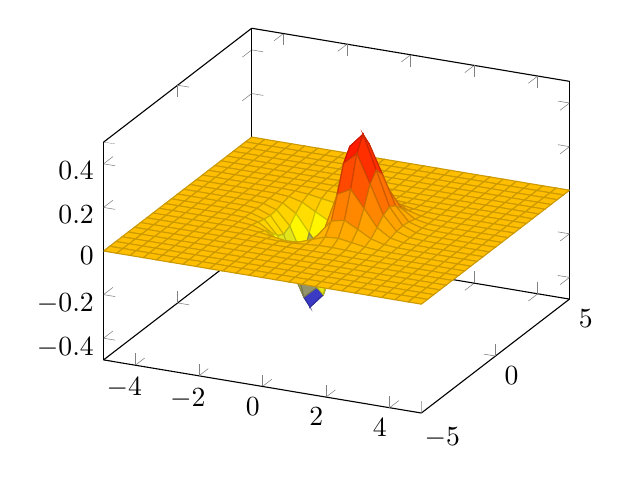
\begin{tikzpicture}
\begin{axis}
\addplot3[
    surf,
]
{exp(-x^2-y^2)*x};
\end{axis}
\end{tikzpicture}
\\\\\\\\Let's plot some more charts:\\\\\\\\
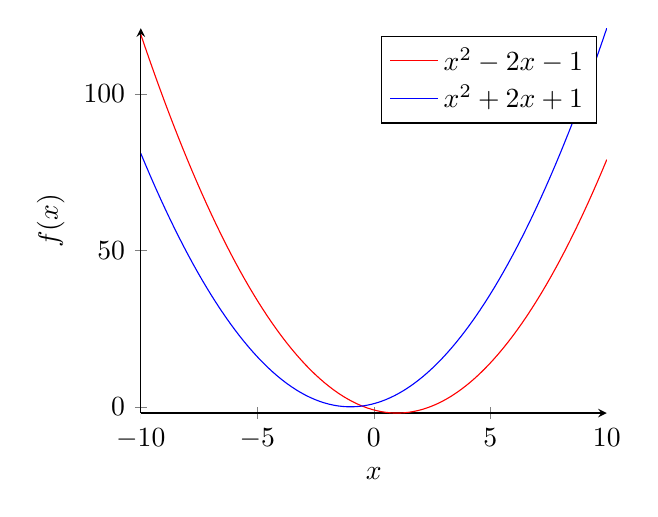
\begin{tikzpicture}
    \begin{axis}[
        axis lines = left,
        xlabel = $x$,
        ylabel = {$f(x)$},
    ]
    %Below the red parabola is defined
    \addplot [
        domain=-10:10, 
        samples=100, 
        color=red,
    ]
    {x^2 - 2*x - 1};
    \addlegendentry{$x^2 - 2x - 1$}
    %Here the blue parablaa is defined
    \addplot [
        domain=-10:10, 
        samples=100, 
        color=blue,
        ]
        {x^2 + 2*x + 1};
    \addlegendentry{$x^2 + 2x + 1$}
    
    \end{axis}
\end{tikzpicture}
\hskip 40pt
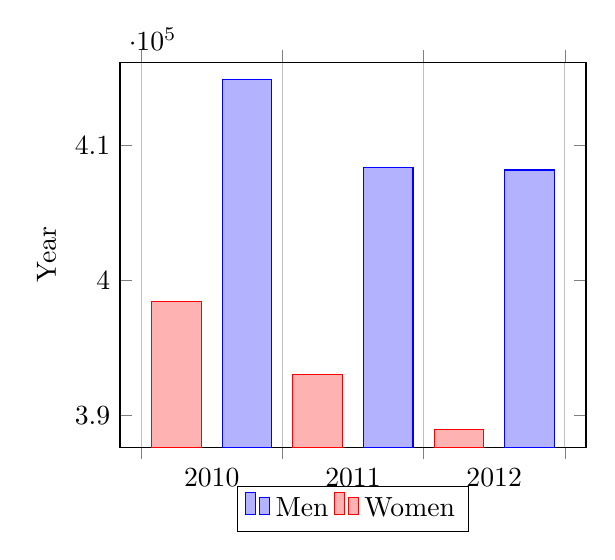
\begin{tikzpicture}  
\begin{axis}[
	x tick label style={
		/pgf/number format/1000 sep=},
	ylabel=Year,
	enlargelimits=0.05,
	legend style={at={(0.5,-0.1)},
	anchor=north,legend columns=-1},
	ybar interval=0.7,
]
\addplot 
	coordinates {(2012,408184) (2011,408348)
		 (2010,414870) (2009,412156)};
\addplot 
	coordinates {(2012,388950) (2011,393007) 
		(2010,398449) (2009,395972)};
\legend{Men,Women}
\end{axis}
\end{tikzpicture}

\newpage
Tips: The blank lines have a meaning in LaTex\\
If I copy the same charts I used in the first row\\
But I introduce a white line between them this happens:\\\\\\\\
\begin{tikzpicture}
\begin{axis}
\addplot[color=red]{exp(x)};
\end{axis}
\end{tikzpicture}
%Here ends the first plot
% This code is the same as the previous 2 charts.
% However if I skip this line they will be in 2 different rows!

\hskip 50pt
%Here begins the 3d plot
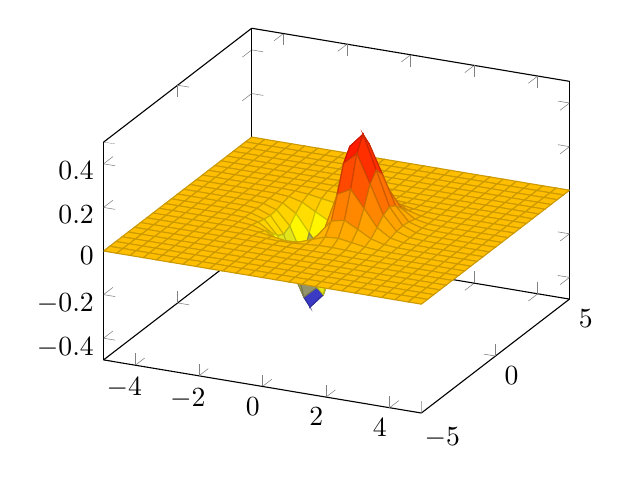
\begin{tikzpicture}
\begin{axis}
\addplot3[
    surf,
]
{exp(-x^2-y^2)*x};
\end{axis}
\end{tikzpicture}\\\\\\\\
3D charts\\\\\\\\
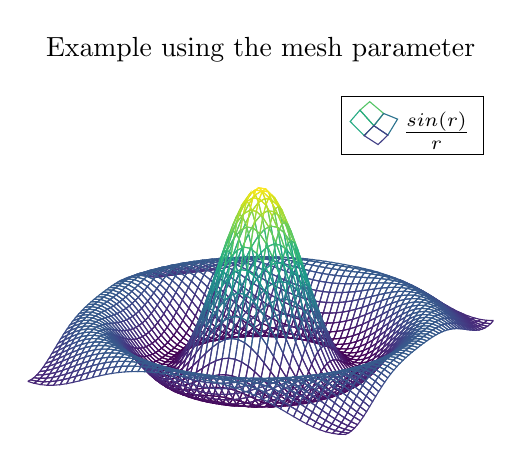
\begin{tikzpicture}
\begin{axis}[
    title=Example using the mesh parameter,
    hide axis,
    colormap/viridis,
]
\addplot3[
    mesh,
    samples=50,
    domain=-8:8,
]
{sin(deg(sqrt(x^2+y^2)))/sqrt(x^2+y^2)};
\addlegendentry{$\frac{sin(r)}{r}$}
\end{axis}
\end{tikzpicture}
\hskip 50pt
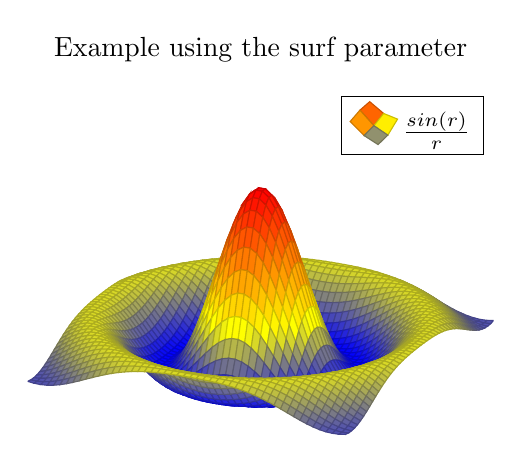
\begin{tikzpicture}
\begin{axis}[
    title=Example using the surf parameter,
    hide axis,
    colormap/hot,
]
\addplot3[
    surf,
    samples=50,
    domain=-8:8,
]
{sin(deg(sqrt(x^2+y^2)))/sqrt(x^2+y^2)};
\addlegendentry{$\frac{sin(r)}{r}$}
\end{axis}
\end{tikzpicture}

\end{document}
